% =====================================================================================
\section{Array analysis}
\label{sec:methods}
% =====================================================================================

The array-level questions (which heaters, at what powers, with what beam) are answered in Python in five steps
(\cref{fig:pipeline}).

\begin{figure}[htbp]
  \centering
  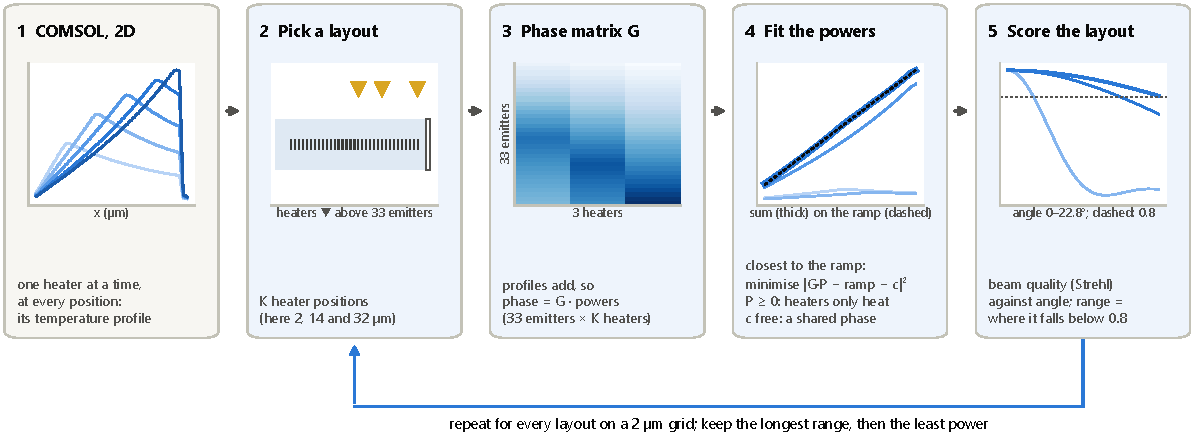
\includegraphics[width=\linewidth]{fig13_pipeline}
  \caption{The analysis. (1)~COMSOL gives the temperature profile of one heater at every position. (2)~A heater
  layout is chosen. (3)~The profiles of its heaters, scaled by $\gamma$, form the phase matrix $G$. (4)~The powers
  are fitted to a target phase profile by non-negative least squares with a free offset. (5)~The layout is scored
  by the Strehl ratio against steering angle; its range ends where this falls below \num{0.8}. Steps 2--5 repeat
  over a grid of layouts. The thumbnails are the slot design's own data.}
  \label{fig:pipeline}
\end{figure}

\subsection{Phase matrix}

$G$ (\cref{eq:G}) is assembled by evaluating the kernel at the \num{33} emitter positions. Kernel columns are
interpolated linearly in heater position; predicting a column from its neighbours \qty{2}{\micro\metre} either
side, twice the largest gap used, reproduces it to within \qty{1}{\percent} of the peak. By superposition
(\cref{sec:superposition}), a heater of width $2m$~\unit{\micro\metre} equals $m$ adjacent \qty{2}{\micro\metre}
heaters at equal power, so wide heaters need no new simulation.

\subsection{Beam quality}
\label{sec:metrics}

The far field is \cref{eq:farfield} evaluated on a fine grid in $\sin\theta$. The figure of merit is the Strehl
ratio, the intensity in the intended direction $u_0=\sin\theta_0$ relative to a perfect ramp aimed there:
\begin{equation}
  S(u_0) \;=\; \Bigl|\frac{1}{N}\sum_{n} \ee^{\,\ii(\phi_n - k_0 x_n u_0)}\Bigr|^{2}.
  \label{eq:strehl}
\end{equation}
The element pattern cancels, and $S$ depends only on the residual phase error. For a small rms residual $\sigma$,
$S\approx\ee^{-\sigma^2}$~\cite{ruze1966}. A beam is accepted when $S\ge0.8$, the usual criterion for a
diffraction-limited beam, which allows $\sigma\approx\qty{0.47}{\rad}$.

\subsection{Heater powers}
\label{sec:fit}

For a target profile $\bm\phi^{\,\mathrm t}$ (a ramp, a parabola or both) the powers and offset minimise the phase
error,
\begin{equation}
  \min_{\bm P\ge 0,\;c}\;\bigl\lVert\, G\bm P - \bm\phi^{\,\mathrm t} - c\,\bm 1 \,\bigr\rVert^{2},
  \label{eq:nnls}
\end{equation}
a non-negative least-squares problem solved with SciPy~\cite{scipy2020}; the constraint
$\bm P\ge0$ expresses that heaters cannot cool. The problem is homogeneous: scaling the target scales the optimal
powers and the residual equally. One fit to a unit ramp therefore gives the powers at every angle,
$\bm P(\theta)\propto\sin\theta$, and $S$ falls monotonically with angle, so each layout has a well-defined
\emph{range}, the largest angle with $S\ge0.8$. Power is quoted per degree, as the power at \ang{1}. The two
steering directions are fitted separately.

\subsection{Heater placement}
\label{sec:placement}

Layouts are ranked by range and then by power. For up to three heaters the search is exhaustive on a
\qty{1}{} or \qty{2}{\micro\metre} grid; for more heaters, a pattern search refines random starts. Symmetric
structures (\stack{standard}, \stack{undercut}) are ranked by their total span over both directions; the
one-sided structures (\stack{slot}, \stack{vacuum}) steer towards $+\theta$ only.

\subsection{Conventional benchmark}
\label{sec:conventional}

The reference is an ideal array of isolated heaters, one per emitter, each supplying its phase modulo $2\pi$:
\begin{equation}
  P_\mathrm{conv}(\theta) \;=\; \frac{\Ppi}{\pi}\,\min_{c}\,\sum_{n}\bigl[(n\,\Delta\phi + c)\bmod 2\pi\bigr].
  \label{eq:conv}
\end{equation}
Above about \ang{1.4} the wrapped phases fill $0$--$2\pi$ evenly and $P_\mathrm{conv}\approx0.9\,N\,\Ppi$,
independent of angle. The benchmark ignores crosstalk, calibration power and the fan-in, so it favours the
conventional design. When a published $\Ppi$ is used, the result is our estimate for an array that has not been
built, and is marked as such.

\subsection{Settling time}
\label{sec:settlemethod}

With the step responses $s_{nk}(t)$ of the thermal model, a step in drive from zero gives
$\phi_n(t)=\gamma\sum_k s_{nk}(t)P_k$. The settling time is the time after which $S\ge0.8$ towards the target is
maintained.
